\documentclass[10pt,landscape]{article}

%encoding
\usepackage[T1]{fontenc}
\usepackage[utf8]{inputenc}
\usepackage{lmodern}

%language
\usepackage[english]{babel}

%paper and text body handling
\usepackage{geometry}
\usepackage{setspace}
\usepackage{lettrine}

%graphics
\usepackage{graphicx}
\usepackage[format = plain, labelfont = {bf, it}, textfont = it]{caption}%font settings for captions
\usepackage{xcolor}
\usepackage{pdfpages}
\usepackage{subcaption}
\usepackage{tcolorbox}
\usepackage{multicol}
\usepackage{tikz}
\usetikzlibrary{arrows.meta}
\usetikzlibrary{bending}


%code
%\usepackage{minted}

%math
\usepackage{amsmath}%math
\usepackage{amssymb}%
\usepackage{amsfonts}%
\usepackage{amsthm}%theorems
\usepackage{aligned-overset}
\usepackage{siunitx}
\usepackage{cancel}
\usepackage{braket}
\usepackage{bm}
\usepackage{diffcoeff}
\usepackage{bbold}
% Use the correct ds in diffs
\diffdef{}{
  op-symbol = \mathrm{d},
  op-order-sep = 0 mu
}

%links
\usepackage[colorlinks=true,
            linkcolor=red,
            urlcolor=blue,
            citecolor=gray]{hyperref}


% Specific to this paper
\newcommand{\maj}{\succ}
\newcommand{\majby}{\prec}
%special letters
\newcommand{\R}{\mathbb{R}}
\newcommand{\C}{\mathbb{C}}
\newcommand{\Z}{\mathbb{Z}}
\newcommand{\N}{\mathbb{N}}
\newcommand{\F}{\mathcal{F}}
\newcommand{\PP}{\mathbb{P}}
\newcommand{\EE}{\mathbb{E}}
\newcommand{\idty}{\mathbb{1}}

%functions
\renewcommand{\Re}{\textnormal{Re}}
\renewcommand{\Im}{\textnormal{Im}}
\DeclareMathOperator{\Var}{Var} % Variance
\DeclareMathOperator{\Cov}{Cov} % Covariance
\DeclareMathOperator{\Res}{Res} % Residue
\DeclareMathOperator{\Ker}{Ker} % Kernel
\DeclareMathOperator{\tr}{tr} 	% Trace
\newcommand{\scalprod}[2]{\left\langle#1, #2\right\rangle}
\newcommand{\expval}[1]{\left\langle#1\right\rangle}

\DeclarePairedDelimiter\abs{\lvert}{\rvert}%
\DeclarePairedDelimiter\norm{\lVert}{\rVert}%

% Swap the definition of \abs* and \norm*, so that \abs
% and \norm resizes the size of the brackets, and the
% starred versions do not.
\makeatletter
\let\oldabs\abs
\def\abs{\@ifstar{\oldabs}{\oldabs*}}
%
\let\oldnorm\norm
\def\norm{\@ifstar{\oldnorm}{\oldnorm*}}
\makeatother

%symbols
% for := as
\newcommand*{\defeq}{%
    \mathrel{%
        \vcenter{%
            \baselineskip0.5ex \lineskiplimit0pt \hbox{\scriptsize.}\hbox{\scriptsize.}%
        }%
    }%
    =%
}


%settings

%spacing
\renewcommand{\arraystretch}{1.2}
\setlength{\arraycolsep}{3pt}

%units
\sisetup{
   output-decimal-marker = {,},
   exponent-product = \ensuremath{\cdot}
}

%text
\makeatletter
   \newlength{\textSize}
   \setlength{\textSize}{\f@size pt}
\makeatother
%\setlength{\parindent}{0 pt}             % No indentation on new paragraph
%\setstretch{1.15}


%paper and text body
\geometry{
	top=0.5cm,
	bottom=0.5cm,
	left=0.5cm,
	right=0.5cm,
   a4paper,
   centering,
}


%lettrine settings
\setcounter{DefaultLines}{3}


\renewcommand{\vec}{\bm}

\newcommand{\topiccolor}{green}
\renewcommand{\section}[2]{%
	\renewcommand{\topiccolor}{#2}
	\begin{tcolorbox}[boxsep=0.5mm, left=1mm, right=1mm, top=0mm, bottom=0mm,
		colback=#2!30, colframe=#2, arc is angular]%
		\centering \textbf{#1}%
	\end{tcolorbox}%
	\nopagebreak%
}
\newcommand{\cbf}[1]{\textcolor{\topiccolor!80!black}{\textbf{#1}}}
\newcommand{\cunderbrace}[2]{%
	\begingroup
		\color{\topiccolor}%
		\underbrace{\color{black}#1}_{\color{\topiccolor}#2}%
	\endgroup
}

\begin{document}

\begin{multicols*}{3}
\begin{tcolorbox}[colframe=black, colback=white]
\centering \large Plasma Physics with Applications\\
\small David Hambr\ae{}us \& Ida Ekmark
\end{tcolorbox}

\section{What is a plasma}{gray}
A plasma is defined via the \cbf{ionization degree} $\alpha$ defined as the
fraction of ionized particles. At $\alpha > 0.01$ we say it is 
\cbf{fully ionized}, while for smaller $\alpha$:s its 
\cbf{weakly / partially ionized}.
One important property of a plasma is the ability to quickly screen out changes
in the electric potential, so called \cbf{Debye Screening}.
Debye screening is described by the \cbf{Debye Length} and \cbf{Debye potential}
\begin{align*}
	\lambda_{\rm D} &= \sqrt{\frac{\varepsilon_0 k_{\rm B} T}{n_0e^2}}\\
	\phi_{\rm D} &= \frac{q}{4\pi\varepsilon_0 r}\exp\left(-\frac{r}{\lambda_{\rm D}}\right),
\end{align*}
(p. 4 -- 5).
With the plasma frequency $\omega_{\rm p}=n_0e^2/m_e\varepsilon_0$, the collision frequency $\nu$ and the macroscopic dimension of the plasma $L$, the definition of a plasma requires
\begin{align*}
	\lambda_{\rm D} &\ll L\\
	\frac{4\pi}{3}\lambda_{\rm D}^3n_0 &\gg 1\\
	\nu \ll &\omega_{\rm p}.
\end{align*}

\section{Single particles in EM-field}{orange}

The most fundamental equation of motion for a charged particle in an EM-field is
the \cbf{Lorentz Force Equation}:
\[
	m \diff{\vec v}{t} = q(\vec E + \vec v \times \vec B)
\]
A constant, nonzero E-field with no B-field gives constant acceleration along
$\vec E$. A constant, nonzero B-field with no E-field gives rise to helical
motion with \cbf{cyclotron frequency} $\omega_{\rm c} = \abs{q} B / m$ and
\cbf{Larmor radius} $r_{\rm L} = v_\perp / \omega_{\rm c}$ (p. 8 -- 9, trick is to divide velocity 
into one component parallel and one perpendicular to $\vec B$).
In this circular orbit we have the current and magnetic moment
\begin{align*}
	I&=\frac{\abs q \omega_{\rm c}}{2\pi}=\frac{1}{2\pi}\frac{q^2B}{m}\\
	\mu&=I\pi r_{\rm L}^2=\frac{mv_\perp^2}{2B}=\abs{\frac{q r_{\rm L} v_\perp}{2}},\ \vec \mu = \frac{q\vec r_{\rm L} \times \vec v_\perp}{2}.
\end{align*}
A constant, nonzero B-field with a constant force $\vec F$ gives a constant
acceleration from the component of $\vec F$ along the B-field, while the
component perpendicular to $\vec B$ gives rise to a constant \cbf{drift velocity}
\[
	\vec v_D = \frac1q \frac{\vec F_\perp \times \vec B}{B^2}
\]
(p. 11, trick is to divide $\vec v_\perp$ into a constant drift velocity 
$\vec v_{\rm D}$ and a varying component $u$ which solves the case without a force).
An \emph{inhomogeneous} B-field gives rise to the so called \cbf{grad B drift}.
The motion parallel to the B-field lines is governed by
\[
	m \diff{\vec v_\parallel}{t} = - \mu \nabla_\parallel B,
\]
and for the motion perpendicular we get a drift velocity
\[
	\vec v_{\nabla B} = \frac\mu q \frac{\vec B \times \nabla B}{B^2} = \frac{mv_\perp^2}{2qB^2}\frac{\vec B \times \nabla B}{B}
\]
in addition to the Larmor rotation, just like before (p. 13 -- 16).
\begin{center}
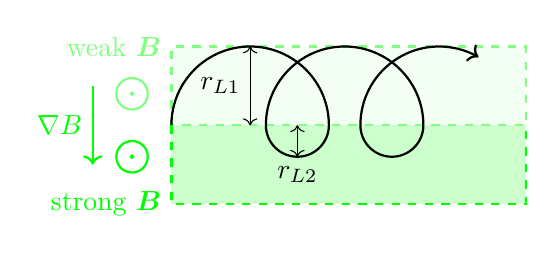
\begin{tikzpicture}[thick]
	\draw[draw=\topiccolor, dashed, fill=\topiccolor!20] (0,0) rectangle (4.5,-1);
	\draw[color=\topiccolor] (-0.5,-0.4) circle[radius=0.2]
		circle[radius=0.014];
	\node at (0,-1) [anchor=east, color=\topiccolor] 
		{strong $\vec B$};

	\draw[draw=\topiccolor!50, dashed, fill=\topiccolor!5] (0,0) rectangle (4.5,1);
	\draw[color=\topiccolor!50] (-0.5,0.4) circle[radius=0.2]
		circle[radius=0.014];
	\node at (0,1) [anchor=east, color=\topiccolor!50] 
		{weak $\vec B$};

	\draw[->, color=\topiccolor] (-1, 0.5) -- node[anchor=east]{$\nabla B$}
		(-1, -0.5);

	\draw[->] (0,0) 
		arc[start angle=180, end angle=0, radius=1]
		arc[start angle=0, end angle=-180, radius=0.4]
		arc[start angle=180, end angle=0, radius=1]
		arc[start angle=0, end angle=-180, radius=0.4]
		arc[start angle=180, end angle=60, radius=1];
	\draw[thin, <->] (1,0) -- node[anchor=east]{$r_{L1}$} (1,1);
	\draw[thin, <->] (1.6,0) -- (1.6,-0.4) node[anchor=north]{$r_{L2}$};

\end{tikzpicture}
\end{center}
When the magnetic field lines are curved, $\abs B$ cannot be constant 
according to Maxwell's equations. 
Thus this such a magnetic field must be inhomogenous and this gives rise
both to a \cbf{grad B drift} and a \cbf{curvature drift}
\begin{align*}
	\vec v_{\rm c} &= \frac{mv_\parallel^2}{qB^2}\frac{\vec B \times \nabla B}{B}\\
	\implies \vec v_{\nabla B} + \vec v_{\rm c} &= \frac{m}{qB^2}\left(\frac12 v_\perp^2 + v_\parallel^2\right)\frac{\vec B \times \nabla B}{B},
\end{align*}
(p. 19).
The final relevant drift velocity is the \cbf{polarization drift} occuring in a slowly varying electric field
\begin{equation*}
	\vec v_{\rm p} = \frac{m}{qB^2} \diff{\vec E}{t}.
\end{equation*}
For a inhomogeneous magnetic field constant in time the magnetic moment is 
invariant (p. 23). 
For a slowly varying magnetic field , this is also true which is called
the first adiabatic invariant (p. 44 -- 45).
The second adiabatic invariant is the integral 
\begin{equation*}
	J = \oint v_\parallel ds
\end{equation*} 
(p. 46 -- 47).

\section{The Vlaslov and Boltzmann equations}{green}

Firstly we define a \cbf{distribution function}, $f(\vec r, \vec v, t)$.
This gives the expected number of particles occupying the volume in
phase space $\dl \vec r \dl \vec v$ around the point $(\vec r, \vec v)$
at time $t$.
To understand how this $f$ evolves argue that the rate of change of the
number of particles inside some volume in phase space $\Omega$ must
be the flux of particles through the walls.
\[
	\diffp*{\int_\Omega f \dl \vec r \dl \vec v}{t}
	= -\int_{\partial_r \Omega} f \vec v \cdot \hat n_r \dl S_r
	-\int_{\partial_v \Omega} f \vec a \cdot \hat n_v \dl S_v.
\]
$\partial_r \Omega$ means the boundry of $\Omega$ in r-space.
Plopping the $\diffp{}{t}$ into the integral and using Gauss' theorem to
make the surface integral a volume integral we obtain
\[
	\dl \vec r \dl \vec v 
	\left[\diffp f t + \diffp{}{\vec r} \cdot \vec v f
	+ \diffp{}{\vec v} \cdot \vec a f
	\right]
	=0,
\]
which has to be true for all volumes, meaning that the integrand has
to be 0 everywhere.
Further noting that $\diffp{}{r} \cdot \vec v = 0$ and plugging in the
Lorentz force for the acceleration we get the \cbf{Vlaslov equation}
\[
	\diffp f t + \vec v \cdot \diffp{f}{\vec r} 
	+ \frac q m(\vec E + \vec v \times \vec B) \cdot \diffp{f}{\vec v} = 0.
\]
The LHS is really the change of $f$ along a particle trajectory (if you let
$\vec r(t)$ and $\vec v(t)$ be the particle position and velocity at time t),
so you can let $f$ be the sum of a bunch of delta functions and reduce this to
the particle description of the plasma.
But this would not be very useful, instead we let $f$ be some smooth
distribution.
This is okay if the collective effect of far away particles are more important
than the effects of collisions.
If we want to include the effects of collisions, we add a mysterious term called
the collision operator to obtain the \cbf{Boltzmann equation}
\[
	\diffp f t + \vec v \cdot \diffp{f}{\vec r} 
	+ \frac q m(\vec E + \vec v \times \vec B) \cdot \diffp{f}{\vec v} 
	= \left(\diffp f t\right)_c.
\]
The $ \left(\diffp f t\right)_c$ is interpreted as the rate of change of $f$
that is due to collisions, and in general we don't have closed form for it.
For plasmas in equilibrium, $\diffp f t = 0$ since they are by definition
stationary in time, and $\left(\diffp f t\right)_c = 0$ as well since the rate
of change due to collisions must also be 0.
The most probablye distribution function describing plasmas in equilibrium
is the Maxwell distribution function
\begin{equation*}
	f_{\rm M} = n \left(\frac{m}{2\pi k_{\rm B}T}\right)^{3/2}\exp\left(-\frac{mv^2}{2k_{\rm B}T}\right),
\end{equation*}
(p. 61 -- 62, trick is to maximise entropy under the constraints that mean velocity is zero, particle density is constant and mean particle energy is constant using Lagrange multipliers).

\section{The two fluid model}{teal}

In this model, we try to simplify the equations above by not caring about the
true $f$, but rather we treat the plasma as a fluid and only care about some of
its moments.
A moment $\expval{\psi}$ is defined as the velocity average
of the function $\psi$:
\[
	\expval{\psi} = \frac1n \int \psi f \dl \vec v,
\]
where $n$ is the density of particles $n(\vec r) = \int f \dl \vec v$.
Using the Boltzmann equation we can derive the \cbf{general moment equation}
\[
	\begin{split}
		\diffp*{(n \expval \psi)}{t} + \nabla \cdot (n \expval{\vec v \psi})
		- \frac{nq}{m} \expval{(\vec E + \vec v \times \vec B) \cdot
		\diffp{\psi}{\vec v}}\\
		= \diffp*{(n\expval{\psi})_c}{t}
	\end{split}
\]
This gives a way of solving the time evolution of these microscopic properties
instead of dealing with $f$ directly.
However, the problem as you can see in the second term is that the equation for
the order $k$ moment contains the order $k+1$ moment.

As an easy example, consider the equation for the zero order moment ($\psi =
1$).
It becomes
\[
	\diff{n_\alpha}{t} + \nabla \cdot (n_\alpha \vec u_\alpha) = 0.
\]
$\vec u_\alpha$ is here the average velocity of the particles of species
$\alpha$ at $\vec r$.
The is basically the continuity equation.
As you can see, it does depend on the average velocity.
The equation for the velocity (first order moment, $\psi=\vec v$) becomes
\begin{multline*}
	n_\alpha m_\alpha \left[ 
		\diffp{\vec u_\alpha}{t} + (\vec u_\alpha \cdot \nabla)\vec u_\alpha
	\right]\\
	= n_\alpha q_\alpha(\vec E + \vec u_\alpha \times \vec B)
	- \cunderbrace{\nabla \cdot \vec \Pi_\alpha}{=\nabla p\text{ if isotropic}}
	+ \sum_{\beta \neq \alpha} P_{\alpha\beta},
\end{multline*}
after a bit of massaging.
Here $\vec P_{\alpha\beta}$ is the effect of collisions between particles of
different species on the average velocity and
$\vec \Pi_\alpha \equiv n_\alpha m_\alpha 
\expval{(\vec v_\alpha - \vec u_\alpha) (\vec v_\alpha - \vec u_\alpha)}$
is the pressure tensor (a central second order moment).
If $f$ is isotropic (I think even if just the velocity distribution is
isotropic, but maybe that is what they meant), then $\nabla \cdot \vec \Pi$
becomes the gradient of the scalar pressure $p=k_B T n$.

\begin{tcolorbox}[title=An aside: wtf is a \textit{pressure tensor}?,
	colframe=\topiccolor!10!white, colback=white, coltitle=\topiccolor]
	If the pressure tensor of a fluid is $\vec \Pi$, then $\vec \Pi \hat n$ is
	the force per unit area on a surface oriented normal to $\hat n$.
	It is the same as the negative of the expectation value of the stress
	tensor: $-\expval{\vec \sigma}$.
	Why is $\vec \Pi = n m \expval{\vec w \vec w}$, where $\vec w = \vec v -
	\expval{\vec v}$? Idk. It's kinda the Irving-kirkwood formula, but I don't
	know where that comes from either.
\end{tcolorbox}

In deriving the second order moment $\expval{mv^2/2}$ (p. 67 -- 69) we get
a Big Boring Expression\texttrademark.
If we ignore the heat exchange between different fluids, and the
\cbf{heat conduction vector}
$\vec Q \equiv n m \expval{\vec w w^2} / 2$
where $\vec w$ is the deviation from the mean velocity,
then some shuffling around gives
\[
	\frac{p_\alpha}{n_\alpha^{5/3}} = \text{const.}
\]
The full equation for the second order moments contain a third order moment and,
for the third a forth and so on.
Somewhere we have to cut it, and here we chose to ignore the third,
thus stopping the chain.

The reason for calling it the \emph{two} fluid model is that we the proceed
to model the plasma using two species: electrons and ions.

\section{MHD / Single fluid model}{lime}

In \cbf{magnetohydrodynamics} (MHD) we treat the plasma as a single conducting
fluid characterized by quantities like the mass density $\rho_m$, the charge
density $\rho$, the center of mass velocity $\vec V$ and the current density
$\vec j$.
These are gotten from the two fluid model in a straight forward manner like
\begin{align*}
	\rho_m &\equiv \sum_\alpha m_\alpha n_\alpha\\
	\rho &\equiv \sum_\alpha q_\alpha n_\alpha\\
	\vec V &\equiv \frac{1}{\rho_m} \sum_\alpha m_\alpha n_\alpha \vec u_\alpha\\
	\vec j &\equiv \sum_\alpha q_\alpha n_\alpha \vec u_\alpha
\end{align*}
The one-fluid equations are then gotten from the two-fluid equations by clever
manipulations, e.g. multiplying the continuity equations by the masses / charges
to get
\begin{align*}
	\diffp{\rho_m}{t} + \nabla \cdot (\rho_m \vec V) = 0\\
	\diffp{\rho}{t} + \nabla \cdot (\vec j) = 0
\end{align*}
or conservation of mass and charge.

Similar manipulations of the two-fluid momentum equations yield
\[
	\rho_m\left(\diffp{}{t} + \vec V \cdot \nabla\right) \vec V
	= \vec j \times \vec B - \nabla \cdot \vec \Pi^*
\]
and the \cbf{Generalized Ohms law}
\[
	bleh\qquad do we even need to write this?
\]

\section{Waves}{red}

What is a wave?
Simply put, when we derive the waves we assume them to be small
perturbations in the underlying equilibrium state.
We also usually look at monochromatic waves:
waves where all of the variables
(density, electric field, mean velocity)
vary with the same frequency:
$X \sim \exp[i (\vec k \cdot \vec r - \omega t)]$.

\section{Maxwells Equations}{gray}

Just for reference, I keep forgetting them all of the time\ldots
\begin{align*}
	\nabla \cdot \vec E &= \frac{\rho}{\varepsilon_0}\\
	\nabla \times \vec E &= -\diffp{\vec B}{t}\\
	\nabla \cdot \vec B &= 0\\
	\nabla \times \vec B &= \mu_0\left(J + \varepsilon_0 \diffp{\vec E}{t}\right)
\end{align*}

\end{multicols*}

\end{document}

